	\documentclass[11pt,a4paper]{article}
\usepackage{geometry}
\usepackage{amsmath}
\usepackage{amssymb}
\usepackage[utf8]{inputenc}  
\usepackage[T1]{fontenc}  
\usepackage{enumitem}
\usepackage{sectsty}
\usepackage{xcolor}
\usepackage{graphicx}
\usepackage{french}
\usepackage{float} 



\usepackage{listings}
 
\definecolor{codegreen}{rgb}{0,0.6,0}
\definecolor{codegray}{rgb}{0.5,0.5,0.5}
\definecolor{codepurple}{rgb}{0.58,0,0.82}
\definecolor{backcolour}{rgb}{0.95,0.95,0.92}
 
\lstdefinestyle{mystyle}{
    backgroundcolor=\color{backcolour},   
    commentstyle=\color{codegreen},
    keywordstyle=\color{magenta},
    numberstyle=\tiny\color{codegray},
    stringstyle=\color{codepurple},
    basicstyle=\ttfamily\footnotesize,
    breakatwhitespace=false,         
    breaklines=true,                 
    captionpos=b,                    
    keepspaces=true,                 
    numbers=left,                    
    numbersep=5pt,                  
    showspaces=false,                
    showstringspaces=false,
    showtabs=false,                  
    tabsize=2
}
 
\lstset{style=mystyle}




%%%%%%%%%%%%%%%%%%
%% MISE EN PAGE %%
%%%%%%%%%%%%%%%%%%
% Marges
\geometry{hmargin=2.5cm,vmargin=2cm}

% On définit les deux couleurs utilisées
\definecolor{couleur_section}{RGB}{0,0,128}
\definecolor{couleur_subsection}{RGB}{0,128,255}

% On personnalise chacun des titres à l'aide des commandes "sectionfont", "subsectionfont", etc.
\sectionfont{\color{couleur_section} \scshape}
\subsectionfont{\color{couleur_subsection}}
\subsubsectionfont{\itshape}



\begin{document}

    %%%%%%%%%%%%%%%%%%%
    %% PAGE DE GARDE %%
    %%%%%%%%%%%%%%%%%%%
    \begin{titlepage}
        \centering
        
\includegraphics[width=0.40\textwidth]{uca.png}\par\vspace{1cm}
        {\scshape\LARGE Université Clermont Auvergne \par}
        {\scshape École Universitaire de Physique et d'Ingénierie \par}
        \vspace{2cm}
        \noindent\rule{\textwidth}{0.5pt}\par
        {\scshape\Large Etude d'un article scientifique de \textbf{Deep Learning}\par}
        \vspace{0.5cm}
        {\huge\bfseries Context Encoder\par}
        \noindent\rule{\textwidth}{0.5pt}\par
        \vspace{5cm}
        {\Large\itshape Lucas TOURON\par}
        {\Large\itshape Sagaf YOUSSOUF\par}

        \vfill

        % Bottom of the page
        {\large 2019 - 2020\par}
    \end{titlepage}



    %%%%%%%%%%%%%%%%%%%%%%%%
    %% TABLE DES MATIERES %%
    %%%%%%%%%%%%%%%%%%%%%%%%
    \tableofcontents
    \newpage
    
    
    
    %%%%%%%%%%%%%%%%%%%%%%%%
    %% CONTENU DU RAPPORT %%
    %%%%%%%%%%%%%%%%%%%%%%%%
    \section{Résumé de l'article}
    Le \textbf{Context Encoder} est un \textbf{auto-encoder} permettant de faire de l'\textbf{inpainting} à partir d'un réseau de neurones. L'\textbf{inpainting} est le fait de reconstruire une partie manquante dans une image. Un auto-encoder est composé de deux parties : l'encoder et le decoder. Pour cette experimentation, l'encoder peut être remplacé par un autre réseau de neuronne tel que Alexnet.
    \\
    Pour faire cela, cet auto-encoder prend en compte un maximum de \textbf{caractéristiques} de l'image existante. Ce réseau de neuronnes est consitué de plusieurs couches de \textbf{convolution} successives. Il est entrainé à l'aide de la méthode de \textbf{réseaux adverses génératifs}.\\
    La fonction objectif est déterminée de 2 manières différentes : par reconstruction et par GAN. Il est aussi possible de fusionner ces deux méthodes, ce qui s'avère être la méthode la plus aboutie selon plusieurs tests effectués sur différentes bases d'images.
    
    \section{Description de la 	méthode proposée}
    Nous avons définit les \emph{concext-encoder} comme étant des réseaux de neurones convolutifs (CNN) qui prédisent les parties manquantes d’une scène à partir des régions voisines de l’image. L’architecture globale de cette méthode est composée d’un pipeline encodeur/décodeur avec une couche entièrement connectée qui fait office de canal entre l’encodeur et le décodeur.

    \subsection{Le pipeline encoder-decoder}
        Le pipeline prend une image en entrée avec des régions manquantes de taille 227*227 et produit une représentation caractéristique de cette image. L’encoder peut être substitué par n’importe quel architecture réseau comme AlexNet.\\
    La forme des régions manquantes peut varier : un carré au centre de l’image, plusieurs carrés ou encore des formes quelconques.\\
    A la suite, le décodeur prend cette représentation et produit le contenu de l’image manquante. Le décodeur est une suite de couche \emph{UpConv/deconv/frac-strided-conv}. L’encodeur et le décodeur sont liés par un canal de couche \textbf{fully connected}.
        \begin{figure}[H]
            \centering
            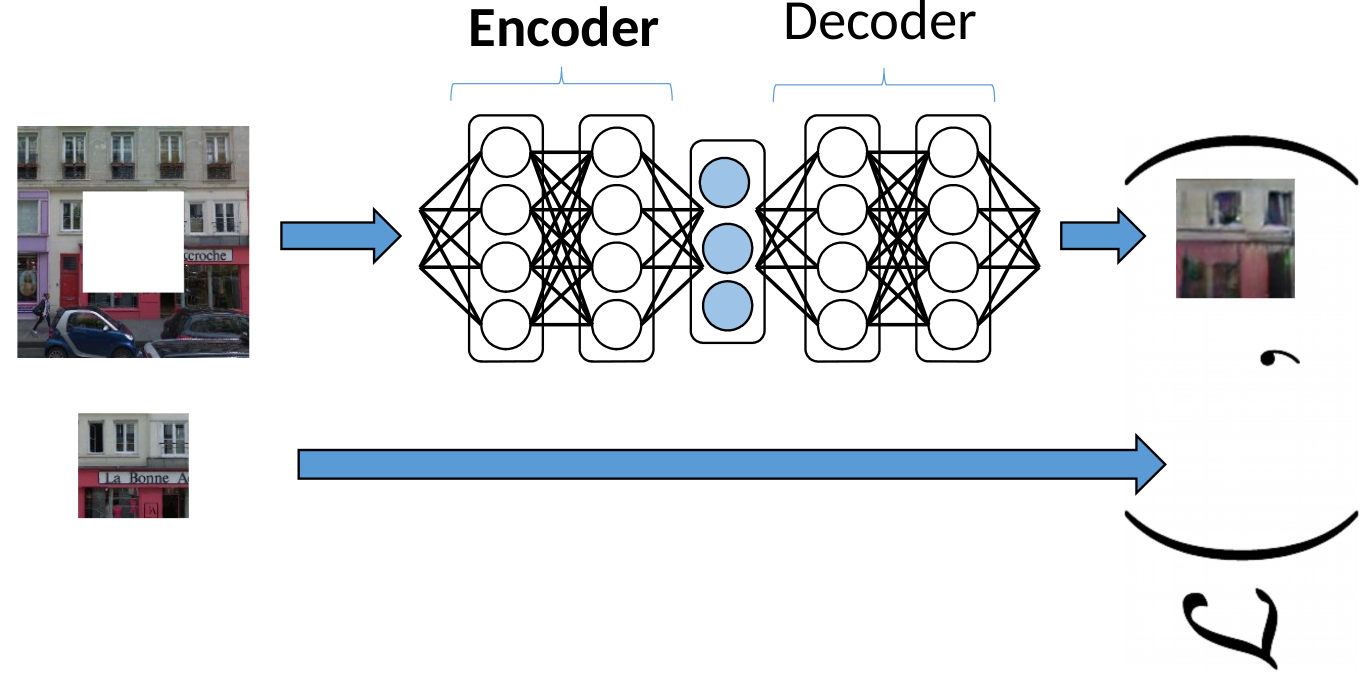
\includegraphics[scale=0.2]{pipeline.png} 
            \caption{Pipeline encoder-decoder}
        \end{figure}

        \subsection{L'encoder}
            L’encodeur utilisé est dérivé de l’architecture d’AlexNet. Il prend une image d’entrée de taille 227*227.\\
            Les 5 premières couches de convolution et les couches de pooling suivantes sont utilisées pour calculer une représentation abstraite de caractéristiques \emph{(de dimensions 6*6*256)}. Puisque l’architecture de l’encodeur est limité à des couches de convolutions, il n’y a aucun moyen de propager les informations à travers les cartes caractéristiques. C’est pour cette raison que l’architecture utilise une couche \emph{fully connected} ou \emph{inner product}. Contrairement aux auto-encodeurs, l’architecture n’essaie pas de reconstruire l’image entière. Les dimensions du latent feature sont donc de 6*6*256 = 9216 pour l’encodeur et le décodeur. En utilisant une couche entièrement connectée, le nombre de paramètres va considérablement augmenter (\textbf{> 100M !}). L’entraînement sera donc très difficile.  Pour y remédier, on utilise une couche \textbf{channel-wise fully connected} décris ci-dessous. 
        
        \subsection{La couche \emph{channel-wise fully connected}}
            Contrairement à une couche entièrement connectée, cette couche n’a pas de paramètres reliant les cartes d’activations. Elle va juste propager l’information à l’intérieur des activations pour chaque carte de caractéristiques.  Le nombre de paramètre de cette couche est \emph{m* n} \emph{(en ignorant les biais)} alors qu'une couche de entièrement connectée dont le nombre de paramètre est de \emph{m* $n^{\text{4}}$}.

        \subsection{Le decodeur}
            La deuxième partie du pipeline est le décodeur. Il génère les pixels de l’image à l’aide des fonctions de l’encodeur.\\
            Comme on l’a déjà précisé, les caractéristiques de l’encodeur et du décodeur sont reliés ensemble à l’aide de la couche \emph{channel-wise fully connected}. Cette couche est suivi d’une série de 5 couches ascendants \emph{(up-convolutional)} avec des filtres appris et des fonctions d’activation ReLU. 
            
        \subsection{Le fonction perte}
            Pour entraîner le context-encoder, on fait une régression au contenu de vérité de terrain de la région manquante de l’image.  Il existe plusieurs façons d’estimer une région d’images manquantes compatible avec le concept de context-encoder. Les auteurs de cet article ont modélisé ce comportement avec une fonction de perte découplée.  Deux types de fonctions de perte ont été étudié :
            \begin{enumerate}[noitemsep]
                \item \textbf{La perte de reconstruction (reconstruction loss L2)}\\
                Cette fonction perte assure la capture de la structure globale de la région manquante et de la cohérence par rapport à son contexte. 
                \item \textbf{L’adversial loss}\\
                L’adversial loss quand à lui tente de faire paraître la prédiction réelle en choisissant un mode particulier dans la distribution. Elle est basés sur les réseaux adverses génératifs (GAN). Il s’agit d’une classe d’algorithme d’apprentissage non-supervisé permettant de générer des images avec une forte degré de réalisme. Cette méthode a été adapté en modélisant le générateur du GAN par le context-encoder. L’approche exploitée dans l’article consiste à conditionner uniquement le générateur et non le discriminateur.
            \end{enumerate}
            L’architecture globale du context-encoder est illustrée par la figure suivante. La perte de reconstruction L2 assure la correctness de l'image et l'Adversarial Loss quand à lui assure la realness de l’image.
            \begin{figure}[H]
                \centering
                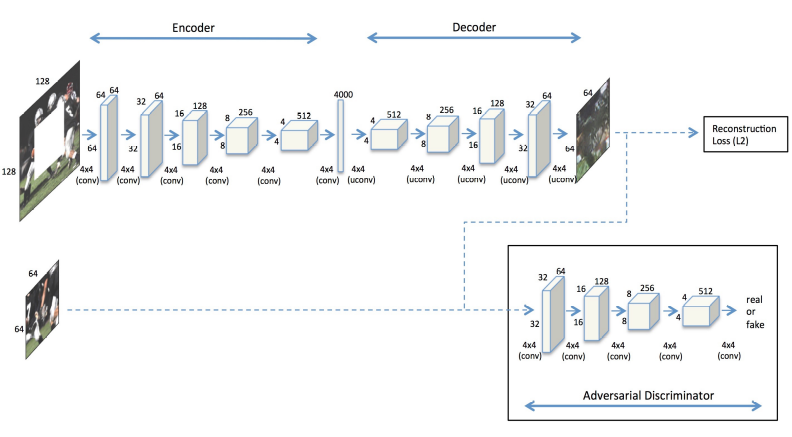
\includegraphics[scale=0.55]{architecture.png} 
                \caption{Architecture du context encoder}
            \end{figure}


            
    \section{Description des tests}
        \subsection{Détails de l'implémentation}
            Le code officiel \emph{(cf annexe 2)} de l’article est implémenté en \texttt{Caffe} et \texttt{Torch}. Pour l’optimisation, c’est la méthode \texttt{ADAM} qui a été utilisé.\\
            Pour des fins de simplicité et pour faire le lien avec les TPs de l’UE de Deep Learning, on utilisera une implémentation écrite en \texttt{Python} avec \texttt{Keras}. Elle est disponible sur Github \emph{(cf annexe 3)}. L'objectif des tests est d’expérimenter les capacités et les limites du context-encoder.
            
        \subsection{L'encoder}                
            \begin{lstlisting}[language=Python, caption=Code Python de l'encoder]
# Encoder
model.add(Conv2D(32, kernel_size=3, strides=2, input_shape=self.img_shape, https://www.xm1math.net/doculatex/listes.htmlpadding="same"))
model.add(LeakyReLU(alpha=0.2))
model.add(BatchNormalization(momentum=0.8))
model.add(Conv2D(64, kernel_size=3, strides=2, padding="same"))
model.add(LeakyReLU(alpha=0.2))
model.add(BatchNormalization(momentum=0.8))
model.add(Conv2D(128, kernel_size=3, strides=2, padding="same"))
model.add(LeakyReLU(alpha=0.2))
model.add(BatchNormalization(momentum=0.8))

model.add(Conv2D(512, kernel_size=1, strides=2, padding="same"))
model.add(LeakyReLU(alpha=0.2))
model.add(Dropout(0.5)) \end{lstlisting}
        
        \subsection{Le decoder}              
            \begin{lstlisting}[language=Python, caption=Code Python du decoder]
# Decoder
model.add(UpSampling2D())
model.add(Conv2D(128, kernel_size=3, padding="same"))
model.add(Activation('relu'))
model.add(BatchNormalization(momentum=0.8))
model.add(UpSampling2D())
model.add(Conv2D(64, kernel_size=3, padding="same"))
model.add(Activation('relu'))
model.add(BatchNormalization(momentum=0.8))
model.add(Conv2D(self.channels, kernel_size=3, padding="same"))
model.add(Activation('tanh'))\end{lstlisting}

        \subsection{Le discriminateur du GAN}              
            \begin{lstlisting}[language=Python, caption=Code Python du discriminateur]
# Discriminateur
model.add(Conv2D(64, kernel_size=3, strides=2, input_shape=self.missing_shape, padding="same"))
model.add(LeakyReLU(alpha=0.2))
model.add(BatchNormalization(momentum=0.8))
model.add(Conv2D(128, kernel_size=3, strides=2, padding="same"))
model.add(LeakyReLU(alpha=0.2))
model.add(BatchNormalization(momentum=0.8))
model.add(Conv2D(256, kernel_size=3, padding="same"))
model.add(LeakyReLU(alpha=0.2))
model.add(BatchNormalization(momentum=0.8))
model.add(Flatten())
model.add(Dense(1, activation='sigmoid'))
model.summary()\end{lstlisting}

    \section{Conclusion}


    %%%%%%%%%%%%%%%%%%%%%%%
    %% TABLE DES FIGURES %%
    %%%%%%%%%%%%%%%%%%%%%%%
    \newpage
    \listoffigures
    \newpage



    %%%%%%%%%%%%%%%%%%
    %% BIBLIOGRAPHY %%
    %%%%%%%%%%%%%%%%%%
    \begin{thebibliography}{9}
        \bibitem{contextencoder} 
            Deepak Pathak, Phillip Krähenbühl, Jeff Donahue, Trevor Darrell, Alexei A. Efros\\
            \textit{Context Encoders: Feature Learning by Inpainting}.\\
            UC Berkeley, CVPR, 2016.
            \\\texttt{https://people.eecs.berkeley.edu/\~{}pathak/context\_encoder}
        \bibitem{github Pathak} 
            Deepak Pathak\\
            \textit{Github de Pathak}.
            \\\texttt{https://github.com/pathak22/context-encoder}
        \bibitem{github Erik Linder Noren} 
            Erik Linder Noren\\
            \textit{Github de Erik Linder Noren}.
            \\\texttt{https://github.com/eriklindernoren/Keras-GAN/tree/master/context\_encoder}
    \end{thebibliography}


\end{document}

